%This is a very basic  BE PROJECT PRELIMINARY template.
%#############################################
%#########Author :  PROJECT###########
%#########COMPUTER ENGINEERING############


\documentclass[oneside,a4paper,12pt]{report}
%\usepackage{showframe}
%\hoffset = 8.9436619718309859154929577464789ptzx
%\voffset = 13.028169014084507042253521126761pt

\fancypagestyle{plain}{%
  \fancyhf{}
  \fancyfoot[CE]{\thepage}
  \fancyfoot[RE]{\thepage}
}
\pagestyle{fancy}
\fancyhead{}
\renewcommand{\headrulewidth}{0pt}
\footskip = 0.625in
\cfoot{}
\rfoot{}

\usepackage[]{hyperref}
\usepackage{tikz}
\usetikzlibrary{arrows,shapes,snakes,automata,backgrounds,petri}
\usepackage{pdfpages}
\usepackage{tabularx}

\usepackage[nottoc,notlot,notlof,numbib]{tocbibind}
\usepackage[titletoc]{appendix}
\usepackage{titletoc}
\renewcommand{\appendixname}{Annexure}
\renewcommand{\bibname}{References}

\setcounter{secnumdepth}{5}

\usepackage{float}
\usepackage{subcaption}
\usepackage{multirow}

\usepackage[ruled,vlined]{algorithm2e}

\begin{document}

\setlength{\parindent}{0mm}
\begin{center}
{\bfseries \fontsize{16}{14} \selectfont  A PRELIMENERY REPORT ON  \\}
 \vspace*{1.5\baselineskip}
{\bfseries \fontsize{16}{14} \selectfont ``SECURE E WALLET ARCHITECTURE USING BCT FEATURES"\\ \vspace*{1.5\baselineskip}}
{\fontsize{12}{12} \selectfont SUBMITTED TO THE SAVITRIBAI PHULE PUNE UNIVERSITY, PUNE\\
IN THE PARTIAL FULFILLMENT OF THE REQUIREMENTS  \\
FOR THE AWARD OF THE DEGREE \\
OF\\	
\vspace*{1\baselineskip}}

{\bfseries \fontsize{14}{12} \selectfont BACHELOR OF ENGINEERING\\
\vspace*{0.6\baselineskip}}

{\bfseries \fontsize{14}{12} \selectfont IN\\
\vspace*{0.6\baselineskip}}

{\bfseries \fontsize{14}{12} \selectfont INFORMATION TECHNOLOGY\\
\vspace*{1\baselineskip}}

{\bfseries \fontsize{12}{12} \selectfont  BY \\
\vspace*{0.5\baselineskip}}

\begin{tabular}{l l}
Jay Pardeshi & 71834755C\\
Jay Sharma & 71834756M\\
Sunil Bhadu & 71917204H\\
Atharva Tribhuwane & 71835034M\\
\end{tabular}

\vspace*{0.7\baselineskip}

{\bfseries \fontsize{14}{12} \selectfont UNDER THE GUIDANCE OF \\
\vspace*{0.5\baselineskip}}

{\bfseries \fontsize{14}{12} \selectfont Prof. Rajesh Tak\\
\vspace*{0.5\baselineskip}}


\includegraphics[width=80pt]{logo} \\
\vspace*{1\baselineskip}
{\bfseries \fontsize{14}{12} \selectfont DEPARTMENT OF INFORMATION TECHNOLOGY  \\}
\vspace*{0.5\baselineskip}

{\bfseries \fontsize{12}{12} \selectfont  Dhole Patil College Of Engineering Pune\\}
\vspace*{0.5\baselineskip}


{\bfseries \fontsize{12}{12} \selectfont Savitribai Phule Pune University \\}
\vspace*{0.5\baselineskip}

{\bfseries \fontsize{12}{12} \selectfont 2021-22\\}

\end{center}

%-----------------------------------------------------------------------------
\newpage
\begin{figure}[ht]
\centering

\includegraphics[width=90pt]{logo}
\end{figure}
{\bfseries \fontsize{14}{12} \selectfont \centerline{CERTIFICATE }
\vspace*{0.5\baselineskip}}

\centerline{This is to certify that the project report entitles }
\vspace*{0.5\baselineskip}

{\bfseries \fontsize{14}{12} \selectfont \centerline{``SECURE E WALLET ARCHITECTURE USING BCT FEATURES"}}
\vspace*{1\baselineskip}

{\bfseries \fontsize{14}{12} \selectfont \centerline{Submitted By }}
\vspace*{0.5\baselineskip}

\begin{center}
\begin{tabular}{l l}
Jay Pardeshi & 71834755C\\
Jay Sharma & 71834756M\\
Sunil Bhadu & 71917204H\\
Atharva Tribhuwane & 71835034M\\
\end{tabular}
\end{center}

\vspace*{0.5\baselineskip}

are bonafide student of this institute and the work has been carried out by him under the supervision of \textbf{Prof. Rajesh Tak} and it is approved for the partial fulfillment of the requirement of Savitribai Phule Pune University, for the award of the degree of Bachelor of Engineering (IT ENGINEERING). \\\\\\


\bgroup
\def\arraystretch{0.5}
\begin{tabular}{c c }
\textbf{Prof. Rajesh Tak} &  \hspace{55 mm} \textbf{Prof. Rahul Ghode} \\								
Internal Guide   &  \hspace{55 mm}Head Of Department \\
Dept. of IT Engineering &	\hspace{55 mm}Dept. IT Engineering
\end{tabular}

\vspace*{4\baselineskip}
\bgroup
\def\arraystretch{0.5}
\begin{tabular}{c c }
 &  \hspace{60 mm} \textbf{Dr. Nihar Walimbe} \\								
 \hspace{5 mm}External Examiner  &  \hspace{60 mm}Principal \\
  &	\hspace{60 mm}DPCOE, PUNE\\
\end{tabular}
\vspace*{0.5\baselineskip}

Place : \\
Date  : 


\thispagestyle{plain}
\setcounter{page}{0}
\frontmatter
\cfoot{Department of IT Engineering 2021-22}
\rfoot{\thepage}


\pagenumbering{Roman}
%\pictack{BE PROJECT TITLE}{Guide Name}

%-------------------------------------------------------------------------------------------------------------
{  \newpage {\bfseries \fontsize{14}{12} \selectfont \centerline{Acknowledgments} 
\vspace*{2\baselineskip}} }

\textit{It gives us great pleasure in presenting the project report on {\bfseries \fontsize{12}{12} \selectfont `SECURE E WALLET ARCHITECTURE USING BCT FEATURES'}.}
\vspace*{1.5\baselineskip}

 \textit{We would like to take this opportunity to thank my internal guide \textbf{Prof. Rajesh Tak} for giving me all the help and guidance we needed. we are really grateful to them for their kind support. Their valuable suggestions were very helpful.} \vspace*{1.5\baselineskip}

 \textit{We are also grateful to \textbf{Prof. Rahul Ghode}, Head of IT Engineering Department, \textbf{DPCOE, PUNE} for his indispensable support, suggestions.}
 \vspace*{3\baselineskip} \\
\begin{tabular}{p{8.2cm}c}
& Jay Pardeshi \\
& Jay Sharma \\
& Sunil Bhadu \\
& Atharva Tribhuwane \\
&(B.E. IT Engg.)
%}
\end{tabular}
% \maketitle
\addcontentsline{toc}{section}{Acknowledgment}



%-----------------------------------------------------------------------------

%%%%%%%%%%%%%%%%%%%%%%%%%%%%%%%%%%%%%%%%%%%%%%%%%%%%%%%%%%%%%%%%%%%%%%%%%%%%%%%%%%%%%%%%%%%%%%%%%%%%%%%%%%%%%%		
{  \newpage {\bfseries \fontsize{14}{12} \selectfont \centerline{Abstract}
\vspace*{2\baselineskip}}}
  \paragraph*{} In 2016, the Indian government, led by Prime Minister Narendra Singh Modi, announced that the nation’s two highest-denomination bank notes would cease to be legal tenders. At the time, the two denominations accounted for roughly 86 percent of cash in circulation in India. People who possessed the banknotes were to deposit them in the bank. With the move, the Indian government aimed to punish tax evaders in retrospect. The logic was that people with hoards of “black money” would have to answer questions if they attempted to deposit the demonetized banknotes. Banking and technology are very closely associated and innovations have changed banking drastically over the period of time.  The digital innovations in the banking sector started with the introduction of money that replaced the barter system and then the gradual replacement of wax seal with digital signatures.  One such disruptive innovation which is changing the banking sector globally is Blockchain Technology (BCT). Blockchain is shared distributed ledger which stores business transaction to a permanent unbreakable chain which can be viewed by the parties in a transaction. Blockchain technology has the potential to disrupt the financial business applications as it provides permanent and tamper proof recording of transactions in a distributed network

Index Terms:- cashless economy, security, distributed database, visual cryptography, hash algorithm,etc.

%-----------------------------------------------------------------------------


\tableofcontents
\listoffigures
\listoftables
\mainmatter
\titleformat{\chapter}[display]
{\fontsize{16}{15}\filcenter}
{
 \bfseries\LARGE\MakeUppercase{\chaptertitlename}~\thechapter}
{1pc}
{\bfseries\LARGE\MakeUppercase}
[\thispagestyle{empty}]
\setlength{\parindent}{11mm}
\chead{  \fontsize{10}{8} \selectfont ``SECURE E WALLET ARCHITECTURE USING BCT FEATURES"}
%---------------------------------------------------------------------------
\chapter{INTRODUCTION}
\section{Overview}
India is currently the seventh-largest economy in the world. It currently has an estimated population of about 1.34 bln people, or about 18 percent of the world’s population, according to the World Economic Forum. Despite its GDP dropping by roughly 5.7 percent in the quarter that ended June of this year, India remains the fastest growing large economy in the world — other than China. If estimates are anything to go by, India will have overtaken China as the world’s most populous country by 2024, which would help solidify its position as the nation with the world’s largest youth population. The World Economic Forum also projects that India’s economy will be the second-largest economy in the world by 2050, with China occupying the first position. Poor as the policy might have been for average Indians, though, there were bright spots for proponents of a cashless economy. The World Economic Forum reported that the number of digital transactions in India increased following the demonetization policy — a plus for the government, who would now have increased ability to track the flow of money within the economy. The growth in digital transaction in India is, in turn, a big plus for Blockchain and cryptocurrency. Just about 0.5 percent of the people in India are into Bitcoin, the cryptocurrency that popularized the Blockchain technology. By inference, if such few people in India know about Bitcoin, it’s safe to say that only about 0.5 percent of India’s population is conversant with Blockchain technology. However, on the national level, a lot of work is going on to integrate Blockchain technology into various sectors of the economy – including the financial and health sectors. In 2016, the Indian bank, ICIC Bank, announced that it had completed a cross-border transaction executed on a Blockchain. In September of this year, the Institute for Development and Research in Banking Technology, or IDRBT, founded by the Reserve Bank of India, announced plans to launch a new Blockchain platform. The Reserve Bank of India is India’s central bank. The announcement followed a report published by the IDRBT in January of this year, that India could use Blockchain to digitize its national currency, the rupee. Given the positives — increased tax payments, for instance — that the demonetization policy in India has yielded through increased digital transactions, it’s plausible that the Indian government will double down on its drive to grow a cashless economy. There are some challenges, but it seems promising. If, as in any place in the world, the Indian government wants to boost its cashless economy, it needs to find lasting solutions to the challenges confronting the propagation of a cashless economy. Some of those challenges include financial inclusion, high setup and transaction costs and transaction times. 
 
\section{Motivation}
The digital innovations in the banking sector started with the introduction of money that replaced the barter system and then the gradual replacement of wax seal with digital signatures.  One such disruptive innovation which is changing the banking sector globally is Blockchain Technology (BCT). Blockchain is shared distributed ledger which stores business transaction to a permanent unbreakable chain which can be viewed by the parties in a transaction. Blockchain technology has the potential to disrupt the financial business applications as it provides permanent and tamper proof recording of transactions in a distributed network.
\section{Problem Definition and Objectives}
1.	If, as in any place in the world, the Indian government wants to boost its cashless economy, it needs to find lasting solutions to the challenges confronting the propagation of a cashless economy. Some of those challenges include financial inclusion, high setup and transaction costs and transaction times.\newline
2.	Due to a considerable segment of the Indian economy remaining informal, there’s still a huge part of the population that doesn’t rely on traditional financial institutions for financial services. Based on the cashless technologies employed today, most people would need a bank account in order to live in a cashless economy — an uphill battle. In essence, for you to run a cashless economy, you’ll need an alternative to traditional financial services.
.
\subsection{Objectives:}


1.	To implement a java based web application.\newline
2.	To implement AES.\newline
3.	To implement block chain.\newline
4.	To implement distributed database system using WLAN.\newline
\section{Project Scope and Limitations}

Project will be developed as a prototype model using JSP and servlet technology. It will run as a local host. System will be communicate through wireless local area network. System communication will be limited in the wireless local area network, but in future if we will host the project using WAN , it can communicate world wide. 
\section{Methodologies of Problem solving}
BCT 
The Blockchain technology almost entirely eliminates the need to belong in the tradition financial system, in order to be financially included. It costs a merchant between Rs 4,000  and Rs 8,000  to set up a card-swiping terminal in India. That is definitely not a problem for big-ticket merchants, but smaller merchants who collectively constitute a big part of the economy might not be happy to pay that much in addition to the subsequent transaction fees. For instance, The Hindu reported in May that Indian consumers are moving back to cash-based transactions, because of remonetization and high digital transaction costs. This makes a case for a cheaper way of conducting digital transactions. Again, Blockchain fits the bill. If a cashless economy is ever going to be the order of the day, it needs to have a real time feature to it. Today’s technologies have done a great job in reducing the wait times between when a transaction is completed and when the funds become accessible. But, it’s not yet at the level where the entire populace will be motivated to go digital. And this is another problem that the Blockchain technology solves brilliantly.



\chapter{LITERATURE SURVEY}
\begin{table}[!htbp]
\begin{center}
\caption{Literature Survey}
\label{tab:Literature Survey}
\def\arraystretch{1.5}
\begin{tabular}{| p{0.5cm} | p{2cm} |p{2cm}| p{2cm} | p{5.5cm} |} \hline
\textbf{Sr. No.} & \textbf{Title} & \textbf{Authors / Year}& \textbf{Advantage} & \textbf{Description} \\ \hline
1. & The Implementation of E-money in Mobile Phone: A Case Study at PT Bank KEB Hana
   & Didik Haryadi ; Harisno ; Victory Haris Kusumawardhana ; Harco Leslie Hendric Spits Warnars2018
   & Cryptography
   & This study aims to analyze the design of e-money, as well as provide some development ideas that must be done related to the implementation of e-money. Here the system uses e payment using QR code and encryption technology.

. \\ \hline

2. & A Landscape of Cryptocurrencies


   & Zhaofang Li ; Qinghua Lu ; Shiping Chen ; Yue Liu ; Xiwei Xu 2019


   & Used Cryptography
   & This study aims to analyze the design of e-money, as well as provide some development ideas that must be done related to the implementation of e-money. Here the system uses e payment using QR code and encryption technology.

. \\ \hline
\end{tabular}
\end{center}
\end{table}

\newpage
\begin{table}[!htbp]
\begin{center}
\def\arraystretch{1.5}
\begin{tabular}{| p{0.5cm} | p{2cm} |p{2cm}| p{2cm} | p{5.5cm} |} \hline
\textbf{Sr. No.} & \textbf{Title} & \textbf{Authors / Year}& \textbf{Advantage} & \textbf{Description} \\ \hline

3. & Security Management and Visualization in a Blockchain-based Collaborative Defense
   & Christian Killer ; Bruno Rodrigues ; Burkhard Stiller 2019


   & BCT
   & This work presents the design of a security management dashboard for BloSS, designed for interactive use by cyber security analysts. This work is about DDos attacks in defense system. \\ \hline

4. & On the Effectiveness of Multi-Token Economies


   & Sean Kang ; Kideok Cho ; Kyle Park 2019
   & BCT
   & This paper addresses the token classification, the reason for adopting multi-token economies and the effectiveness of them. We analyze the Steemit as a representative example of multi-token economies. We describe how the multi-token economy has been working and show the distinctive features of multi-token economies. We also propose the evaluation criteria for multi-token economies. \\ \hline

5. & Digitizing Invoice and Managing VAT Payment Using Blockchain Smart Contract



   & Van-Cam NGUYEN ; Hoai-Luan PHAM ; Thi-Hong TRAN ; Huu-Thuan HUYNH ; Yasuhiko NAKASHIMA 2019


   & BCT
   & This paper proposed implementation of VAT system as an online system using BCT. A distributed database system is used in online system. System can be prevented from hacking using BCT. \\ \hline

\end{tabular}
\end{center}
\end{table}
%NNNNNNNNNNNNNNNNNNNNNNNNNNNNNNNNNNNNNNNNNNNNNNNNNNNNNNNNNNNNNNNNNNNNNNNNNNNNNNNNNNNNNNNNNNNNNNNNNNNNNNNNNNNNNNNNNNNNNN

\chapter{Software Requirement Specification}

%NNNNNNNNNNNNNNNNNNNNNNNNNNNNNNNNNNNNNNNNNNNNNNNNNNNNNNNNNNNNNNNNNNNNNNNNNNNNNNNNNNNNNNNNNNNNNNNNNNNNNNNNNNNNNNNNNNNNNN

\section{Project Scope}
\begin{itemize}
\item To develop prototype model for cashless india using BCT.
\item This model will be run at local host using Glassfish server.
\item BCT features such as decentralization, cryptography and hash codes will be implemented.
\end{itemize}

\section{Assumptions and Dependencies}
\hspace*{0.5cm} This document will provide a general description of project, including user requirements, product perspective, and overview of requirements, general constraints. In addition, it will also provide the specific requirements and functionality needed for this project such as interface, functional requirements and performance requirements.

\subsection{User Classes and Characteristics}
\hspace*{0.5cm} Find the different user classes that you anticipate will use this product. User classes can be differentiated based on use frequency or product functions subset used or technical expertise or privilege levels or educational level and experience. It also describe the pertinent behavior or characteristics of each user class. Few requirements may limited only to specific user classes. Differentiate the very most important or useful user classes for this item or product from those who are less significant to satisfy.

\section{Functional Requirements}
\hspace*{0.5cm} Functional user requirements is nothing but very high-level statements about what the system should and also it should describe clearly an overview of  system services in detail.

\section{External Interface Requirements}
\subsection{User Interfaces}
\hspace*{0.5cm} The user interface or UI for the software should be compatible to be used by any standard browser such as IE, Mozilla or Google chrome. Using this UI user can have access to the system. The UI or user interface can be developed  by using many tool or software package like JFrame.

\subsection{Hardware Interfaces}
\hspace*{0.5cm} A hardware interface is needed to run the software. Java (JDK) and NetBeans compatible hardware is required which is minimal requirement. 

\subsection{Software Interfaces}
\hspace*{0.5cm} It uses Java as the front end programming tool. MySQL has been used as  back end application tool. Latest version of java anything higher than 7.0 can be used. 

\newpage

\section{Non Functional Requirements}
\subsection{Performance Requirements}
\begin{itemize}
\item System can work optimal or faster on 8 GB or more of RAM.
\item The system is targeted to be available all time. Once there is a fatal error or system down, the system will provide understandable feedback to the user.
\end{itemize}

\subsection{Safety Requirements}
\begin{itemize}
\item  The system is designed in modules where errors can be detected.
\end{itemize}

\subsection{Security Requirements}
\begin{itemize}
\item The system is designed in modules where errors can be detected and fixed easily.
\end{itemize}

\subsection{Software Quality Attributes}
\begin{itemize}
\item \textbf{Usability: }\\
\hspace*{0.5cm} This relates to how easily people can use app/website. A measure of usability could be the time it takes for end users to become familiar with my app/website functions, without training or help.
\item \textbf{Reliability:}\\
\hspace*{0.5cm} This can be defined as the available time or UP time of software.
\item \textbf{Performance: }\\
\hspace*{0.5cm} This is essentially how fast app/website works. A performance requirement for the app/website could be start in less than 20 seconds.
\item \textbf{Security :}\\
\hspace*{0.5cm} Say that app/website saves all the previous code and lets you reuse a saved code.
\end{itemize}


\newpage
\section{System Requirements}
\subsection{Database Requirements}
\textbf{MySQL Database}\\
\hspace*{0.5cm} MySQL is on open source database which is mainly a RDBMS i.e. relational database management system. As a database server, primary function of this software is to storing and retrieving data as requested by other from end software applications like java which may  Or may not run either on the same computer or on different computer. This can be across the network either in internet or intranet.

\subsection{Software Requirements}
\begin{enumerate}
\item \textbf{Operating System: } Microsoft Windows 7 and Above
\item \textbf{Programming Language: } Java
\item \textbf{IDE: } Netbeans, Android Studio
\end{enumerate}
\subsection{Hardware Requirements}
\begin{enumerate}
\item \textbf{Processor: } Intel Core I3 or Higher
\item \textbf{RAM: } 4 GB or Higher
\item \textbf{Hard Disk: } 100 GB (min)
\end{enumerate}

\section{Analysis Models: SDLC Model to be applied}
\textbf{SDLC model to be applied}\\
\textbf{Waterfall Model:}\\
\hspace*{0.5cm} The Waterfall Model is among very first and old model of software development life cycle. It is also called as a linear-sequential life cycle model. This is very simple in nature and easy to understand or use. This is step by step method so next step can only be begin once earlier has been completed. This is mainly used for small scale project. Constant or fixed requirement should be there for this type of model. 

\begin{center}
	\begin{figure}[!htbp]
		\centering
		\fbox{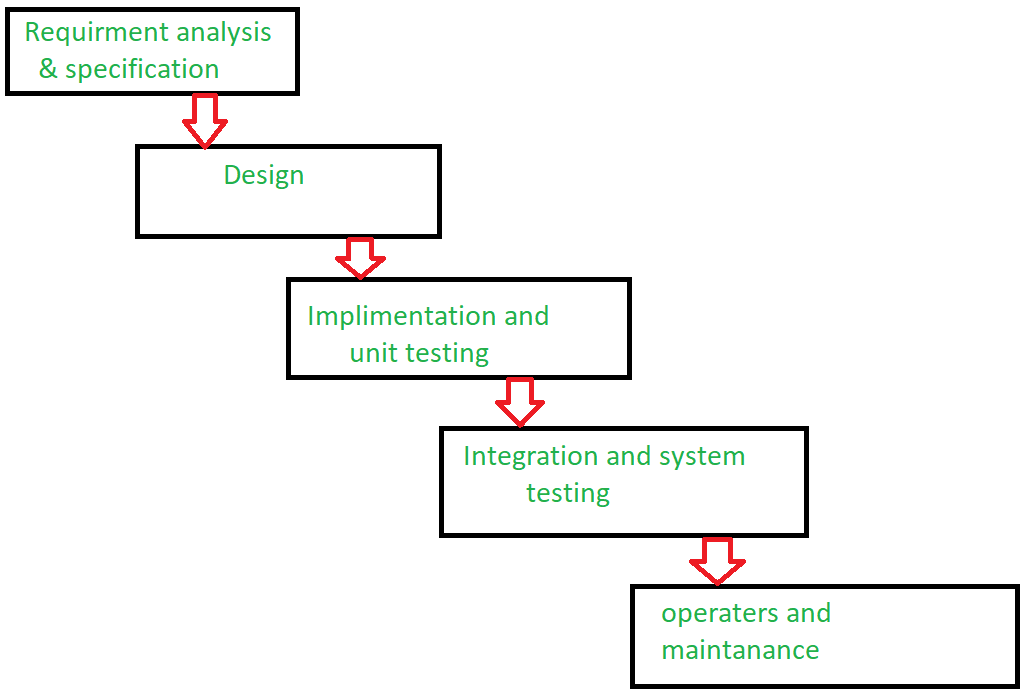
\includegraphics[scale=0.65	]{waterfall}}
	    \caption{Waterfall Model}
	    \label{fig:Waterfall Model}
	\end{figure}
\end{center}

%NNNNNNNNNNNNNNNNNNNNNNNNNNNNNNNNNNNNNNNNNNNNNNNNNNNNNNNNNNNNNNNNNNNNNNNNNNNNNNNNNNNNNNNNNNNNNNNNNNNNNNNNNNNNNNNNNNNNNN

\chapter{System Design}

%NNNNNNNNNNNNNNNNNNNNNNNNNNNNNNNNNNNNNNNNNNNNNNNNNNNNNNNNNNNNNNNNNNNNNNNNNNNNNNNNNNNNNNNNNNNNNNNNNNNNNNNNNNNNNNNNNNNNNN

\section{System Architecture}

\begin{center}
	\begin{figure}[!htbp]
		\centering
		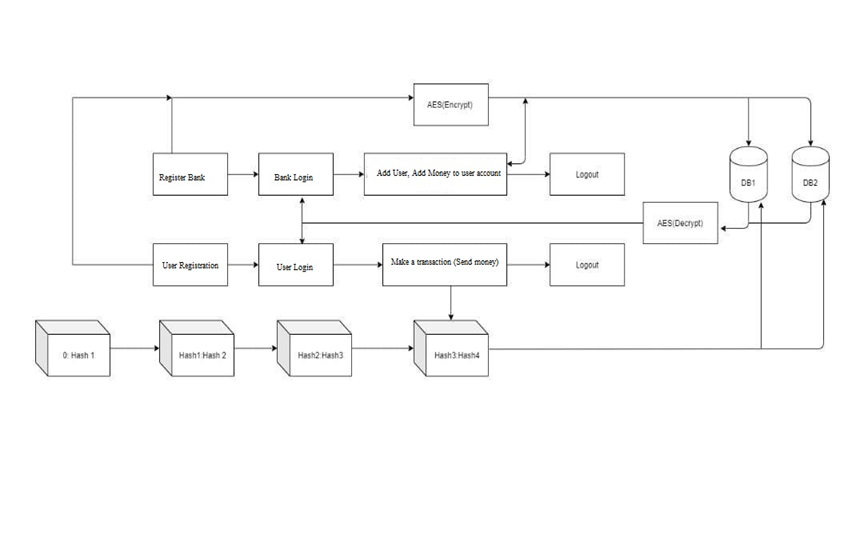
\includegraphics[scale=0.70]{architecture}
        \caption{System Architecture}
	    \label{fig:System Architecture}
	\end{figure}
\end{center}
Whenever any transaction will occur in the system , the record of that transaction is maintained in the form of hash value in a block. Each next block will get attached to the previous block and in this way a virtual block chain will occur. The hash value of a current block is generated using the data of a current block and the hash of the previous block. In this way if any of the block is tempered the subsequent all the block’s hash must be changed . Such multiple copies are maintained at different servers , which will assure the data security and confidentiality.  As everything is through application interface, it will maintain the transparency in transaction.

\newpage

\section{MATHEMATICAL MODEL}

Let
\newline
S be Closed system defined as, S = { Ip, Op, Ss, Su, Fi, A}

To select the input from the system and perform various actions from the set of actions A so that Su state can be attained.
\newline 
S={Ip,Op,Ss,Su,Fi,A}
\newline
Where,
\newline   
IP1={Username,Password, image}
\newline
Set of actions=A={F1,F2,F3,F4}
\newline
Where
\newline
F1= Send Mail
\newline
F2= Merge Images
\newline
F3= Encrypt Database
\newline
F4= Generate Hash
\newline
S=Set of users
\newline
Ss={rest state, registration state, login state}
\newline
Su- success state is successful analysis
\newline
Fi- failure state 
\newline
Objects:
\newline
1)	Input1: Ip1 = {Username, Password}
\newline
2)	Input2 : Ip2= {image from mail}
\newline
1)	Output1 : Op1 = Transaction Record 
\newline
2)	Output2 : Op2 = Encrypted Database
\newline
3)	Output3 : Op3 = Hash Codes.
\newpage
\section{Data Flow Diagrams}
\hspace*{0.5cm} A data flow diagram (DFD) is a graphical representation of the ``flow" of data through an information system, modeling its process aspects. A DFD is often used as a preliminary step to create an overview of the system, which can later be elaborated. DFDs can also be used for the visualization of data processing.  

\subsection{Level 0 Data Flow Diagram}
\begin{center}
	\begin{figure}[!htbp]
		\centering
		\fbox{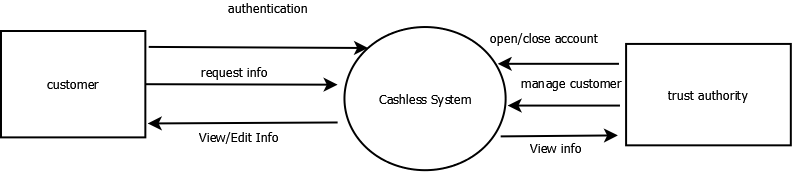
\includegraphics[scale=0.35]{dfd0}}
   	    \caption{Level 0 Data Flow Diagram}
	    \label{fig:Level 0 Data Flow Diagram}
	\end{figure}
\end{center}


\newpage
\subsection{Level 1 Data Flow Diagram}
 \begin{center}
	\begin{figure}[!htbp]
		\centering
		\fbox{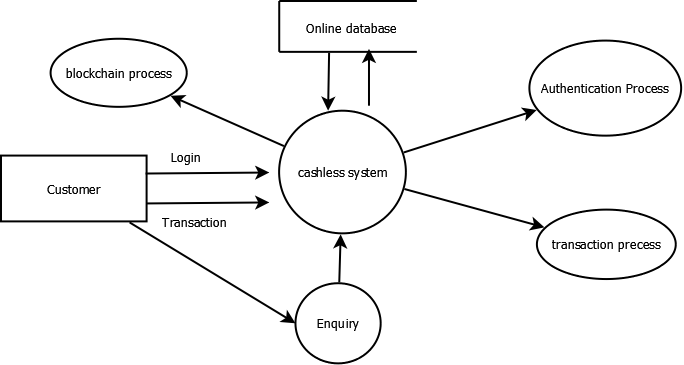
\includegraphics[scale=0.40]{dfd1}}
	    \caption{Level 1 Data Flow Diagram}
	    \label{fig:Level 1 Data Flow Diagram}
	\end{figure}
\end{center}

\newpage
\section{Entity Relationship Diagrams}
\hspace*{0.5cm} An entity relationship diagram (ERD) shows the relationships of entity sets stored in a database. An entity in this context is an object, a component of data. An entity set is a collection of similar entities. These entities can have attributes that define its properties. By defining the entities, their attributes, and showing the relationships between them, an ER diagram illustrates the logical structure of databases.

\begin{center}
	\begin{figure}[!htbp]
		\centering
		\fbox{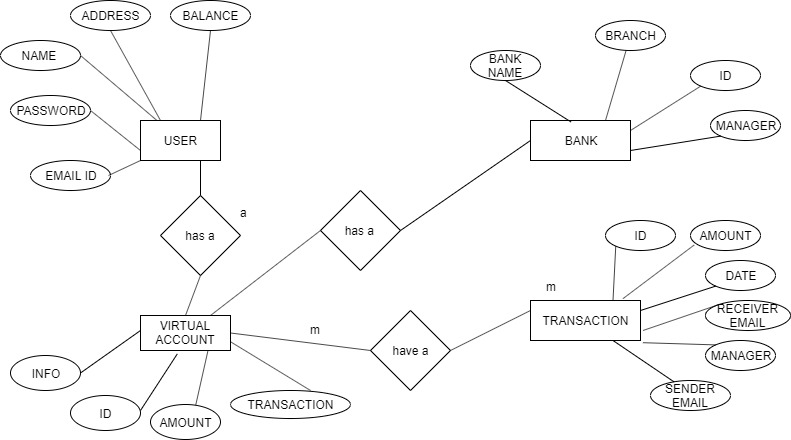
\includegraphics[scale=0.35]{er}}
  	    \caption{Entity Relationship Diagrams}
	    \label{fig:Entity Relationship Diagrams}
	\end{figure}
\end{center} 

\newpage
\section{UML Diagrams}
\subsection{Class Diagram}
\hspace*{0.5cm} A class diagram in the world of Unified Modeling Language or UML can be defined as a type of static structure diagram which mainly defines the structure of a system. It works by showing the system’s classes and their attributes and operations or methods also the relationships among objects.

\begin{center}
	\begin{figure}[!htbp]
		\centering
		\fbox{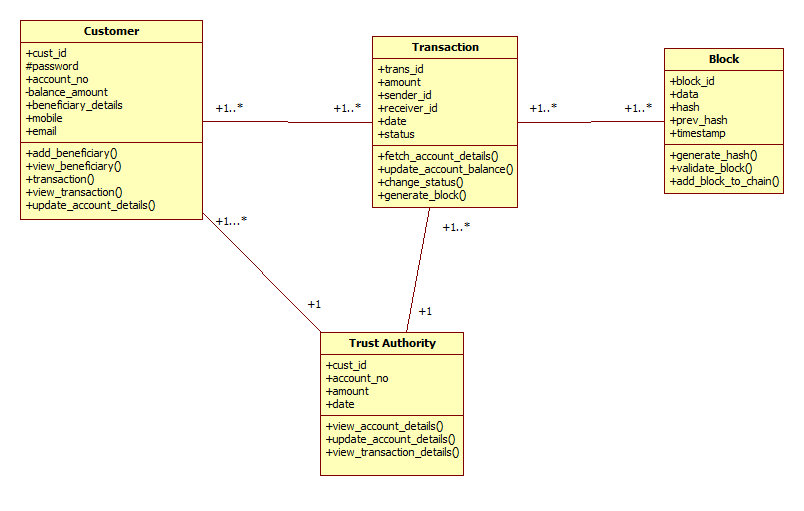
\includegraphics[scale=0.52]{class}}
  	    \caption{Class Diagram}
	    \label{fig:Class Diagram}
	\end{figure}
\end{center}

\newpage
\subsection{Use Case Diagram}
\hspace*{0.5cm} Dynamic behavior is most important aspect to capture the model of any system. Dynamic behavior can be defined as the behavior of the system when it is running or operating. Static behavior is not sufficient to model a system rather dynamic behavior is more important than static behavior.

\begin{center}
	\begin{figure}[!htbp]
		\centering
		\fbox{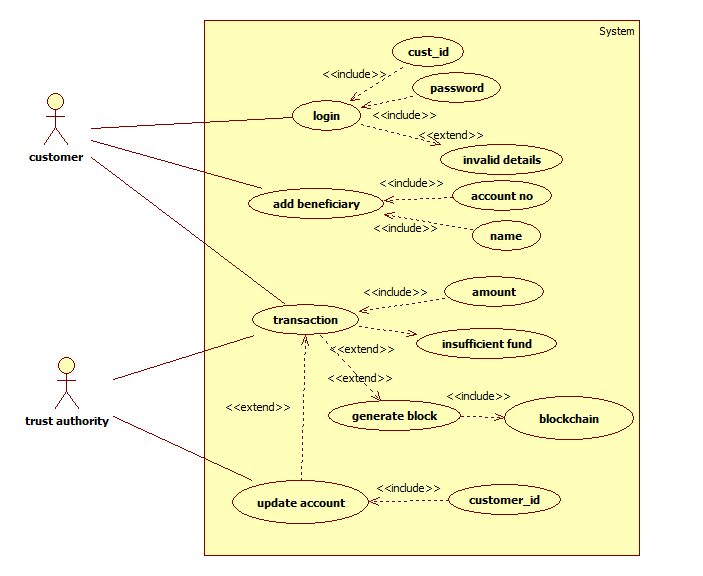
\includegraphics[scale=0.55]{usecase}}
	    \caption{Use Case Diagram}
	    \label{fig:Use Case Diagram}
	\end{figure}
\end{center}

\newpage
\subsection{Sequence Diagram}
\hspace*{0.5cm} Sequence diagrams can be used to provide a graphical representation of object  interactions or object coordination over the time. These basically displays a actor or user, and the objects and components they interact with in the execution of a use case. The sequence diagrams displays the own of messages from one object to another object, and as such correspond to the methods and events supported by a class/object.

\begin{center}
	\begin{figure}[!htbp]
		\centering
		\fbox{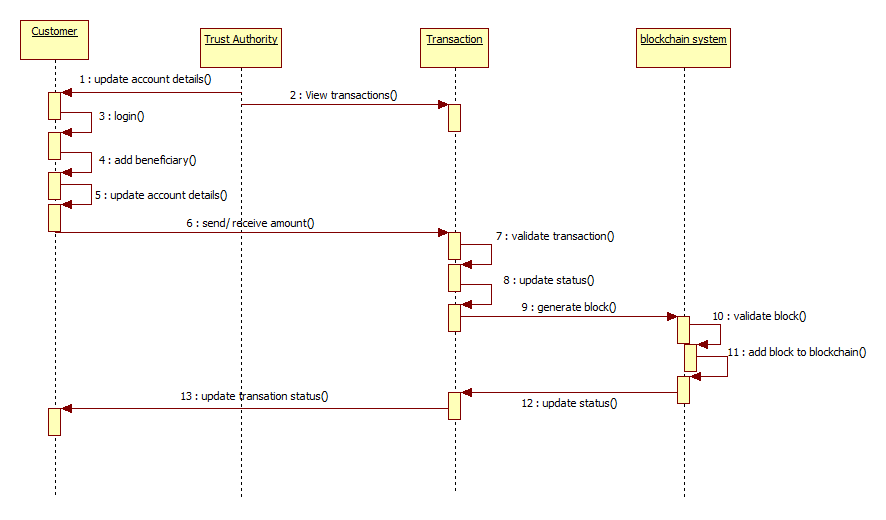
\includegraphics[scale=0.50]{sequence}}
 	    \caption{Sequence Diagram}
	    \label{fig:Sequence Diagram}
	\end{figure}
\end{center}

\chapter{PROJECT PLAN}
\def\arraystretch{1.3}
  \begin{tabular}{|c|c|p{9.2cm}|}
  \hline    
\textbf{Phase}	&\textbf{Task}	&\textbf{Description}	\\ \hline	   
Phase 1 &Analysis &Analyze the information related to Project Topic \\ \hline
Phase 2 & System Design &Assign the module and design the process flow Control \\ \hline
Phase 3 &Implementation &Implement the code for all the modules and integrate all the modules \\ \hline
Phase 4 &Testing &Test the code and overall process weather the process works
properly Test the code and over all process weather the process works properly \\ \hline
Phase 5 &Maintenance & Modification of a software product after delivery to improve performance or maintainability. \\ \hline
\end{tabular}


\newpage
\subsection{Reconciled Estimates}
\section{Project Estimate}
{\renewcommand{\arraystretch}{2}%
	\begin{table}[!htbp]
   
				\begin{tabular}{ |p{1cm}|p{4cm}|p{6cm}|  }
 \hline
 Sr.No. & Milestone Name & Milestone Description\\ 
 \hline
 1. & Requirement Analysis & Complete specification of system \\ 
 \hline
2. & High level design & Identify the modules and the different  entities and their relationships\\
 \hline
 3. & Detailed design & GUI design, program specification etc \\ 
 \hline
4. & Build & Writing code for different modules\\
\hline
5.	& Testing  & Test the different modules together  \\
\hline
6. & Final Review and Deployment & Checking all the requirements are fulfilled \\
\hline
\end{tabular}
\caption{Project Estimate}
	\label{tab:hreq}
\end{table}

\newpage
\subsection{COCOMO Model}
Cocomo (Constructive Cost Model) is a regression model based on LOC, i.e number of Lines of Code. It is a procedural cost estimate model for software projects and often used as a process of reliably predicting the various parameters associated with making a project such as size, effort, cost, time and quality. It was proposed by Barry Boehm in 1970 and is based on the study of 63 projects, which make it one of the best-documented models. The key parameters which define the quality of any software products, which are also an outcome of the Cocomo are primarily Effort \& Schedule:
\begin{itemize}
\item Effort: Amount of labor that will be required to complete a task. It is measured in person-months units.\
\item Schedule: Simply means the amount of time required for the completion of the job, which is, of course, proportional to the effort put. It is measured in the units of time such as weeks, months.\\
\end{itemize}
\
Different models of Cocomo have been proposed to predict the cost estimation at different levels, based on the amount of accuracy and correctness required. All of these models can be applied to a variety of projects, whose characteristics determine the value of constant to be used in subsequent calculations. These characteristics pertaining to different system types are mentioned below.\\

Boehm’s definition of organic, semidetached, and embedded systems:
\begin{enumerate}
\item Organic – A software project is said to be an organic type if the team size required is adequately small, the problem is well understood and has been solved in the past and also the team members have a nominal experience regarding the problem.\
\item Semi-detached – A software project is said to be a Semi-detached type if the vital characteristics such as team-size, experience, knowledge of the various programming environment lie in between that of organic and Embedded. The projects classified as Semi-Detached are comparatively less familiar and difficult to develop compared to the organic ones and require more experience and better guidance and creativity. Eg: Compilers or different Embedded Systems can be considered of Semi-Detached type.\
\item Embedded – A software project with requiring the highest level of complexity, creativity, and experience requirement fall under this category. Such software requires a larger team size than the other two models and also the developers need to be sufficiently experienced and creative to develop such complex models.\
\end{enumerate}

\ All the above system types utilize different values of the constants used in Effort Calculations. Types of Models: COCOMO consists of a hierarchy of three increasingly detailed and accurate forms. Any of the three forms can be adopted according to our requirements. These are types of COCOMO model:
\begin{enumerate}
\item Basic COCOMO Model
\ The first level, Basic COCOMO can be used for quick and slightly rough calculations of Software Costs. Its accuracy is somewhat restricted due to the absence of sufficient factor considerations.\\


The basic COCOMO model estimates the software development effort using only lines of code.\\

\begin{center} $ E=a(KLOC)^b $\\
\end{center}
newline Where,\\
 E is the efforts applied by person in months, a = 3.0 and b = 1.12 , then KLOC=2.25\\
 Hence Efforts = 3.0 (1.8)1.12,\\
 E = 5.79 Person-month\\
 E = 6 Person-month\\
 Total of 6 Person-Month are required to complete the project successfully.\\

\begin{center} $ D=cb(E)^d b$\\
\end{center}
Where,\\
 D = Development time in chronological months, cb = 2.5 and db = 0.35, and E =6 Person-Month\\
 Hence, Development Time= 2.5 (1.8)0.35\\
 D = 3.07 months\\
 The approximate duration of project is 3 months.\\

 P = E/D\\
 Where,\\
 P = Number of persons to accomplish project.\\
Hence, Number of Persons required completing the project\\
 P = 6/3\\
 P = 2 persons\\
 Therefore 2 persons are required to successfully complete the project on schedule.\\

\item Intermediate COCOMO Model
\ Intermediate COCOMO takes these Cost Drivers into account and Detailed COCOMO additionally accounts for the influence of individual project phases, i.e in case of Detailed it accounts for both these cost drivers and also calculations are performed phase wise henceforth producing a more accurate result. These two models are further discussed below.
\item Detailed COCOMO Model
\ In detailed cocomo, the whole software is divided into different modules and then apply COCOMO in different modules to estimate effort and then sum the effort.\
\end{enumerate}

 Project Cost-\\

The model followed is the Constructive Cost Model(COCOMO) for estimating the effort required in completing the project. Like all the estimation models, the COCOMO Model requires sizing information. This information can be specified in the form of:
\begin{itemize}
\item Object Point
\item Function Point
\item Lines of source Code (KLOC) for our project, This work uses the sizing information in the form Lines of Source Code.
\item Total lines of code for our project, KLOC =1.8K (approx.).
\item Cost of each person per month, Cp=Rs.11,000/- (Per person-month)\\
 So, $ C=3 \times Cp=3 \times 11000= 33,000- $
\end{itemize} 
Therefore, the cost pf project is 33,000+10000(cost of camera approx) = 43,000/- (approx).\\

\subsection{Reconciled Estimates}
The part of the project will be hardware, which need to implement in our system on besides, also need to estimates the cost of the application which are designing keeping in mind the following factor:
\begin{itemize}
\item	Its market demand, what it has got to offer to the customer
\item Its relevance in the current world.
\item The extent to which it can adhere to its objective of secured data transmission.
\end{itemize}

\subsection{Project Resources}
1.  Designer: To design system and perform requirement gathering.

2.Developer: To develop system and provide to tester for testing

\newpage
\section{Risk Management}:
\subsection*{Risk Identification}
For risks identification, review of scope document, requirements specifications and schedule is done. Answers to questionnaire revealed some risks. Each risk is cate- gorized as per the categories mentioned in [?].You can refereed following risk iden- tification questionnaire.

1.	Have top software and customer managers formally committed to support the project?
Answer : Yes

2.	Are end-users enthusiastically committed to the project and the system/product to be built?
Answer : Yes

3.	Are requirements fully understood by the software engineering team and its customers?
Answer : Yes

4.	Have customers been involved fully in the definition of requirements?
Answer : Yes

5.	Do end-users have realistic expectations?
Answer : Yes

6.	Does the software engineering team have the right mix of skills?
Answer : Yes

7.	Are project requirements stable?
Answer : Yes

8.	Is the number of people on the project team adequate to do the job?
Answer : Yes

9.	Do all customer/user constituencies agree on the importance of the project and on the requirements for the system/product to be built?
Answer : Yes

5.2.2	NP Hard

A problem is NP-hard if solving it in polynomial time would make it possible to solve all problems in class NP in polynomial time. Some NP-hard problems are also in NP (these are called ”NP-complete”), some are not. If you could reduce an NP problem to an NP-hard problem and then solve it in polynomial time, you could

solve all NP problems. Also, there are decision problems in NP-hard but are not NP-complete, such as the infamous halting problem

5.2.3	Risk Analysis

•	Technical Risk:
The probability of loss incurred through the execution of a technical process in which the outcome is uncertain. Untested engineering, technological or manufacturing procedures entail some level technical risk that can result in the loss of time, resources, and possibly harm to individuals and facilities. Like mobile phone battery off, network error in user and server, multiple requests at time.
•	Operational Risk:
Operational risk is the prospect of loss resulting from inadequate or failed procedures, systems or policies. Employee errors. Systems failures. Fraud or other criminal activity. Any event that disrupts business processes. Like user registration, login, send request to service provider.
\newline
\newline
•	Schedule Risk:
Schedule risk is the risk that the project takes longer than scheduled. It can lead to cost risks, as longer projects always cost more, and to performance risk, if the project is completed too late to perform its intended tasks fully.
\newline
\newline
•	Business Risk:
Business risk is the possibilities a company will have lower than anticipated profits or experience a loss rather than taking a profit. Business risk is influ- enced by numerous factors, including sales volume, per-unit price, input costs, competition, and the overall economic climate and government regulations.


\newpage
\section{Project Schedule}:
\subsection{Project task set}
Major Tasks in the Project stages are:
\newline

\def\arraystretch{1.5}
  \begin{tabular}{| p{3cm} | p{3cm} |p{3cm}|}
\hline
\textbf{Priority (High to low)}	&\textbf{Risks}	&\textbf{Back-up plan}	 \\ \hline  
1	&Schedule	&Overtime	    \\ \hline 
2	&Operational	&Validation	   \\ \hline  
3	&Business	&Marketing	    \\ \hline 
4	&Technical	&-	  \\ \hline 
\end{tabular}
\newline\newline\newline
•	Task 1: Requirement Gathering\newline
•	Task 2: Literature Survey\newline
•	Task 3: System Design\newline
•	Task 4: Functionality Implementation\newline
•	Task 5: Testing


\newpage
\subsection{Timeline Chart}
\begin{center}
	\begin{figure}[!htbp]
	
	\fbox{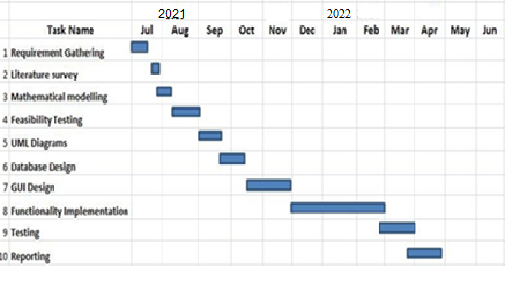
\includegraphics[width=15cm, height=10cm]{plan1}}
		  \caption{Timeline Chart}
	 
	\end{figure}
\end{center} 


\newpage
\section{Team Organization}
\subsection{Team Structure}
Whatever activities are done related to the project that we all showing all details log to our guide. All the reporting are noted to the guide.

\begin{table}[!htbp]
\begin{center}
\def\arraystretch{1.5}
  \begin{tabular}{| c | p{6cm} | c |}
\hline
\textbf{Work Task}	&\textbf{Description}	&\textbf{Duration} \\ \hline
Literature Search	&Related  work  done  for  conceptual  data similarity	&6 weeks \\ \hline
System analysis	&Critical analysis and comparison of technologies  studied  and  results  achieved  in research	&4 weeks \\ \hline
Design and Planning	&Modeling and design and dataset searching or creation	&8 weeks \\ \hline
Implementation	&Divided into phases	& \\ \hline
Phase A	&Implementation module 1	&2 weeks \\ \hline
Phase B	&Implementation module 2	&2 weeks \\ \hline
Phase C	&Implementation module 3	&2 weeks \\ \hline
System Testing	&Test system quality, fix errors if any and improve if needed. Test system for different data sets	&3 weeks \\ \hline
Final Report	&Prepare and upload Initial Report	&2 weeks \\ \hline
Initial Report	&Prepare and upload Initial Report	&2 weeks \\ \hline
\end{tabular}
 \caption {Time line Chart}
 \label{tab:Timeline Chart}
\end{center}
\end{table}
\newpage
\chapter{Project Implementation}
\section{Overview of Project Modules}
BCT: First and foremost, blockchain is a public electronic ledger built around a P2P system that can be openly shared among disparate users to create an unchangeable record of transactions, each time-stamped and linked to the previous one. Every time a set of transactions is added, that data becomes another block in the chain (hence, the name). Blockchain can only be updated by consensus between participants in the system, and once new data is entered it can never be erased. It is a write-once, append-many technology, making it a verifiable and auditable record of each and every transaction.
Famer will transfer the products to the agent through the application interface, agent in turn will transfer any product to another agent through application interface only. Also the record of each and every transaction will be maintained at different places which will maintain transparency also the database is secured through AES. System login is secured through visual cryptography.

\newpage
\section{Tools and Technologies Used:}
JDK 1.8 Installation
1.	Double click jdk-8-ea-bin-b32-windows-i586 to run the installation program.
JDK License dialog displayed. Accept the license in order to install JDK.

2.	The JRE Custom setup dialog enables you to choose a custom directory for JRE Files.
3.	The complete dialog indicates a successful installation.

Net Beans IDE 7.3.1 Installation
To install the software:

1.	After the download completes, run the installer. For Windows, the installer executable file has the .exe extension. Double-click the installer file to run it.
2.	If you downloaded the All bundle, you can customize your installation. Per- form the following steps at the Welcome page of the installation wizard:
a.	Click Customize.
b.	In the Customize Installation dialog box, make your selections.

•	At the Welcome page of the installation wizard, click Next. At the License agreement page, review the license agreement, click the acceptance check box, and click Next. At the JUnit License Agreement page, decide if you want to install JUnit and click the appropriate option, click Next. At the NetBeans IDE installation page, do the following:
•	Accept the default installation directory for the NetBeans IDE or specify an- other directory. Note: The installation directory must be empty and the user profile you are using to run the installer must have read/ write permissions for this directory.
•	Accept the default JDK installation to use with the NetBeans IDE or select   a different installation from the drop-down list. If the installation wizard did not find a compatible JDK installation to use with the Net-Beans IDE, your JDK is not installed in the default location. In this case, specify the path to an installed JDK and click Next, or cancel the current installation. After installing the required JDK version you can restart the installation.

•	If you are installing Apache Tomcat, on its installation page, accept the default installation directory or specify another installation location. Click Next.
•	At the Summary page, verify that the list of components to be installed is correct and that you have adequate space on your system for the installation.
•	Click Install to begin the installation.
•	At the Setup Complete page, provide anonymous usage data if desired, and click Finish.

MySQL Database

Microsoft SQL Server is a relational database management system developed by Mi- crosoft. As a database server, it is a software product with the primary function of storing and retrieving data as requested by other software applications which may run either on the same computer or on another computer across a network (includ- ing the Internet). Microsoft markets at least a dozen different editions of Microsoft SQL Server, aimed at different audiences and for workloads ranging from small single-machine applications to large Internet-facing applications with many concur- rent users.

\newpage
\section{Algorithm Details:}
Algorithm:

\subsection{AES}
AES is used to encrypt the database.\newline
The encryption process uses a set of specially derived keys called round keys. 
These are applied, along with other operations, on an array of data that holds exactly one block of data, the data to be encrypted. 
This array we call the state array.\newline


STEPS:\newline


\begin{itemize}
\item Derive the set of round keys from the cipher key.
\item Initialize the state array with the block data (plaintext).
\item Add the initial round key to the starting state array.
\item Perform nine rounds of state manipulation.\newline
\item Perform the tenth and final round of state manipulation
\item Copy the final state array out as the encrypted data (ciphertext).

\end{itemize}

\subsection{MD5:Hash Function} 

Step 1.Append Padding Bits. The message is "padded" (extended) so that its length (in bits) is congruent to 448, modulo 512. ...\newline
Step 2. Append Length. ...\newline
Step 3. Initialize MD Buffer. ...\newline
Step 4. Process Message in 16-Word Blocks. ...\newline
Step 5. Output.\newline
In cryptography, MD5 (Message-Digest algorithm 5) is a widely used cryptographic hash function with a 128-bit hash value. \newline
As an Internet standard (RFC 1321), MD5 has been employed in a wide variety of security applications, and is also commonly used to check the integrity of files. 
An MD5 hash is typically expressed as a 32 digit hexadecimal number.



\chapter{Conclusion}:

Thus we are going to implement a prototype web based software application in Java for application of BCT for cashless economy . We will implement  block chain features such as:
1.	Decentralization
2.	Hash Algorithm
3.	Encrypted Database.
Thus it is possible to track every transaction in cashless system using BCT. Also the system can be transparent using BCT. 

\section{Future Scope}

In future we will try for sponsorship from government and will implement a project on large scale with some domain and hosting space online.

\section{Applications}

1.	Farmers\newline
2.	Government Organizations\newline
3.	Banking Sector.\newline
4.	Educational System\newline



%-----------------------------------------------------------------------------------------------------------

%\section{Analysis Models: SDLC Model to be applied}
%\begin{itemize}
%\item \textbf{Waterfall Model}\\
%The Waterfall Model was first Process Model to be introduced. It is also referred to as a linear-sequential life cycle model. It is very simple to understand and use. In a waterfall model, each phase must be completed fully before the next phase can begin. This type of model is basically used for the for the project which is small and there are no uncertain requirements. At the end of each phase, a review takes place to determine if the project is on the right path and whether or not to continue or discard the project. In this model the testing starts only after the development is complete. In waterfall model phases do not overlap.
%\begin{center}
%	\begin{figure}[!htbp]
%		\centering
%		\fbox{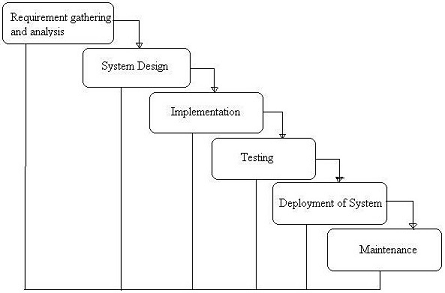
\includegraphics[scale=1]{wt}}
%	  \caption{Waterfall Model}
%	  \label{fig:Waterfall Model}
%	\end{figure}
%\end{center}
%\newpage
%\item \textbf{Applications}
%\begin{enumerate}
%\item This model is simple and easy to understand and use.
%\item It is easy to manage due to the rigidity of the model,each phase has specific deliverables and a review process.
%\item  In this model phases are processed and completed one at a time. Phases do not overlap.
%\item Waterfall model works well for smaller projects where requirements are very well understood.
%\end{enumerate}
%\end{itemize}
%\newpage
%\section{System Implementation Plan}
%\begin{center}
%	\begin{figure}[!htbp]
%		\centering
%		\fbox{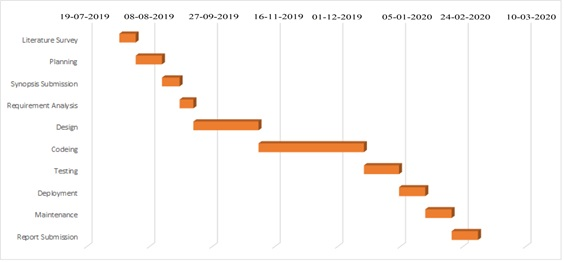
\includegraphics[width=15cm, height=10cm]{plan}}
%	  \caption{Project Plan}
%	  \label{fig:Project Plan}
%	\end{figure}
%\end{center} 


%--------------------------------------------------
\chapter{REFERENCES}
\begin{enumerate}
\item F. Lv and S. Chen, "Research on Establishing a Traceability System of Quality and Safety of
Agricultural Products Based on Blockchain Technology," Rural Finance Research, vol. 12, pp.
22-26, 2016


\item Y. Yang and Z. Jia, "Application and Challenge of Blockchain Technology in the Field of Agricultural Internet of Things,― Information Technology, vol. 258, pp. 24-26, 2017.

\item S. Nakamoto, "Bitcoin: A peer-to-peer electronic cash system,― Consulted, 2008.

\item Y. Yuan and F. Y. Wang, "Blockchain: The State of the Art and Future Trends," Acta Automatica Sinica, 2016.

\item Y. Yuan, T. Zhou, A. Y. Zhou, Y. C. Duan, and F. Y. Wang, "Blockchain Technology: From Data Intelligence to Knowledge Automation," Zidonghua Xuebao/acta Automatica Sinica, vol. 43, pp 1485-1490, 2017.
\item Y.-b. Zhang, "The New Ecosystem of Cross-border E-commerce between EU and China based
on Blockchain," China Business And Market, vol. 32, pp. 66-72, 2018.


\item T. Hong, "Accelerating the Application of Blockchain in the Field of Agricultural Products E -
commerce in China," Journal of Agricultural Information, pp. 18-20, 2016.


\item Y. Yuan and F.-Y. Wang, "Parallel Blockchain: Concept, Methods and Issues," IEEE Acta Automatica Sinica, vol. 43, pp. 1703-1712, 2017.

\item Andreas M A. Mastering Bitcoin: Unlocking Digital Cryptocurrencies. O'Reilly Media, 2014

\item Jerry B, Andrea C. Bitcoin: A Primer for Policymakers. Mercatus Center, George Mason University, 2013.

\end{enumerate}

\begin{appendices}
\chapter{}
\begin{itemize}

\item Definitions: P, NP, NP-Hard, NP-Complete Problems:

\item P Class of problems: Solutions to P class of problems have  deterministic algorithms running  in polynomial.
\item NP Class of problems: Solutions to NP class of problems have non-deterministic algorithms running in polynomial.
\item NP-Hard class of problems: A problem is in NP-Hard class if an already proved NP-Hard problem reduces to it.
\item NP-Complete class of problems: A problem is NP-Complete if it is NP-Hard and it is NP  (i.e. there exists a non-deterministic algorithm running in polynomial time which solves it).

Therefore, our system is NP-Complete. Hence it Is Feasible.

\end{itemize}

\begin{center}
	\begin{figure}[!htbp]
		\centering
		\fbox{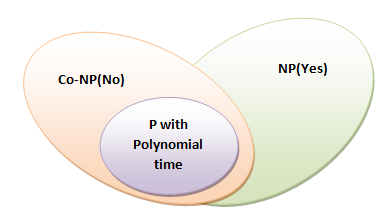
\includegraphics[scale=0.80]{np1}}
   	    \caption{NP Problem}
	    \label{fig:NP Problem}
	\end{figure}
\end{center}

\begin{itemize}




\item What is NP?
•	"NP" means "we can solve it in polynomial time if we can break the normal rules of step-by-step computing".
\item What is NP-Complete?
•	Since this amazing "N" computer can also do anything a normal computer can, we know that "P" problems are also in "NP".
•	So, the easy problems are in "P" (and "NP"), but the really hard ones are *only* in "NP", and they are called "NP-complete".
•	It is like saying there are things that People can do ("P"), there are things that Super People can do ("SP"), and there are things *only* Super People can do ("SP-complete").
\item NP-Complete:
We have use Bloom filtering for detection of packet drop attack whether it is drop by itself or by hacker.  
Hence the ‘P’ is NP-Complete in this case.


\end{itemize}


\begin{center}
	\begin{figure}[!htbp]
		\centering
		\fbox{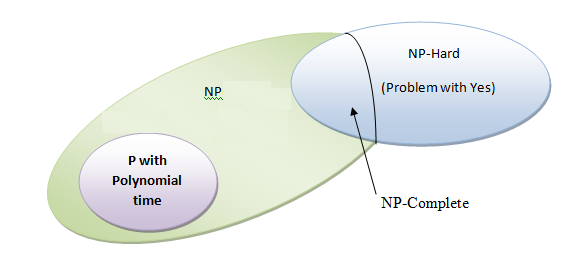
\includegraphics[scale=0.80]{np2}}
   	    \caption{NP Problem Complete}
	    \label{fig:NP Problem Complete}
	\end{figure}
\end{center}

\end{appendices}
\end{document}
%-------------------------------------------------------------------
